\chapter{Setting up a Replica Server (Stratum 1)}
\label{sct:replica}

While a \cvmfs\ Stratum 0 repository server is able to serve clients directly, a large number of clients is better be served by a set of Stratum 1 replica servers.
Multiple Stratum 1 servers improve the reliability, reduce the load, and protect the Stratum 0 master copy of the repository from direct accesses.
Stratum~0 server, Stratum~1 servers and the site-local proxy servers can be seen as content distribution network.
Figure~\ref{fig:stratum1} shows the situation for the repositories hosted in the cern.ch domain.

\begin{figure}
	\begin{center}
		\resizebox{\textwidth}{!}{%\documentclass[a4paper, 11pt]{article}\usepackage{tikz,ifthen}\usetikzlibrary{circuits.logic.US,arrows,positioning,shapes,topaths,calc,fit,backgrounds,matrix,shadows,decorations.pathreplacing,decorations.text,trees}\usepackage[margin=2cm]{geometry}\begin{document}\sf


\begin{tikzpicture}
	\colorlet{rwcolor}{blue}
	\colorlet{publiccolor}{blue}
	\colorlet{mirrorcolor}{black}
	\colorlet{proxycolor}{gray}
	\tikzset{
		rw/.style={very thick,rwcolor},
		public/.style={very thick, publiccolor},
		mirror/.style={thick, mirrorcolor, fill=white},
		replication/.style={thick, ->},
		repltree/.style={%edge from parent fork down, 
			fill=red!30,rounded corners,
			edge from parent={red,-o,thick,draw}}
%		raa/.style={component, draw= contextcolor, text= contextcolor},
%		slc/.style={component, draw=cernvmcolor, text=cernvmcolor},
%		kernel/.style={component, draw=cernvmcolor, text=cernvmcolor},
%		fuse/.style={component, draw=cernvmcolor, text=cernvmcolor},
%		context/.style={component, draw= contextcolor, text=contextcolor},
%		cvmfs/.style={component, draw=cvmfscolor, text=cvmfscolor},
%		httpd/.style={anchor=south west},
%		key/.style={font=\footnotesize}
	}

	\def\rinner{2.25cm}
	\def\router{4cm}
	\def\rmirror{1.5cm}
	\def\websize{1cm}

	
	\begin{scope}
		[grow cyclic, thick, proxycolor,
			level 1/.style={level distance=16mm,sibling angle=60}, 
			level 2/.style={level distance=8mm,sibling angle=45}, 
			level 3/.style={level distance=4mm,sibling angle=30}]
		
		\coordinate[rotate=-90, yshift=\router+\rmirror*0.5] % going down 
			child foreach \x in {1,2,3}
				{child foreach \x in {1,2,3} 
					{child foreach \x in {1,2,3}}};
	\end{scope}
	
	\begin{scope}
		[rotate=180,
		  grow cyclic, thick, proxycolor,
			level 1/.style={level distance=16mm,sibling angle=60}, 
			level 2/.style={level distance=8mm,sibling angle=45}, 
			level 3/.style={level distance=4mm,sibling angle=30}]
		
		\coordinate[rotate=-90, yshift=-\router-\rmirror*0.5] % going down 
			child foreach \x in {1,2,3}
				{child foreach \x in {1,2,3} 
					{child foreach \x in {1,2,3}}};
	\end{scope} 


	\node (rw) at (0,0) {\parbox{3cm}{\centering\small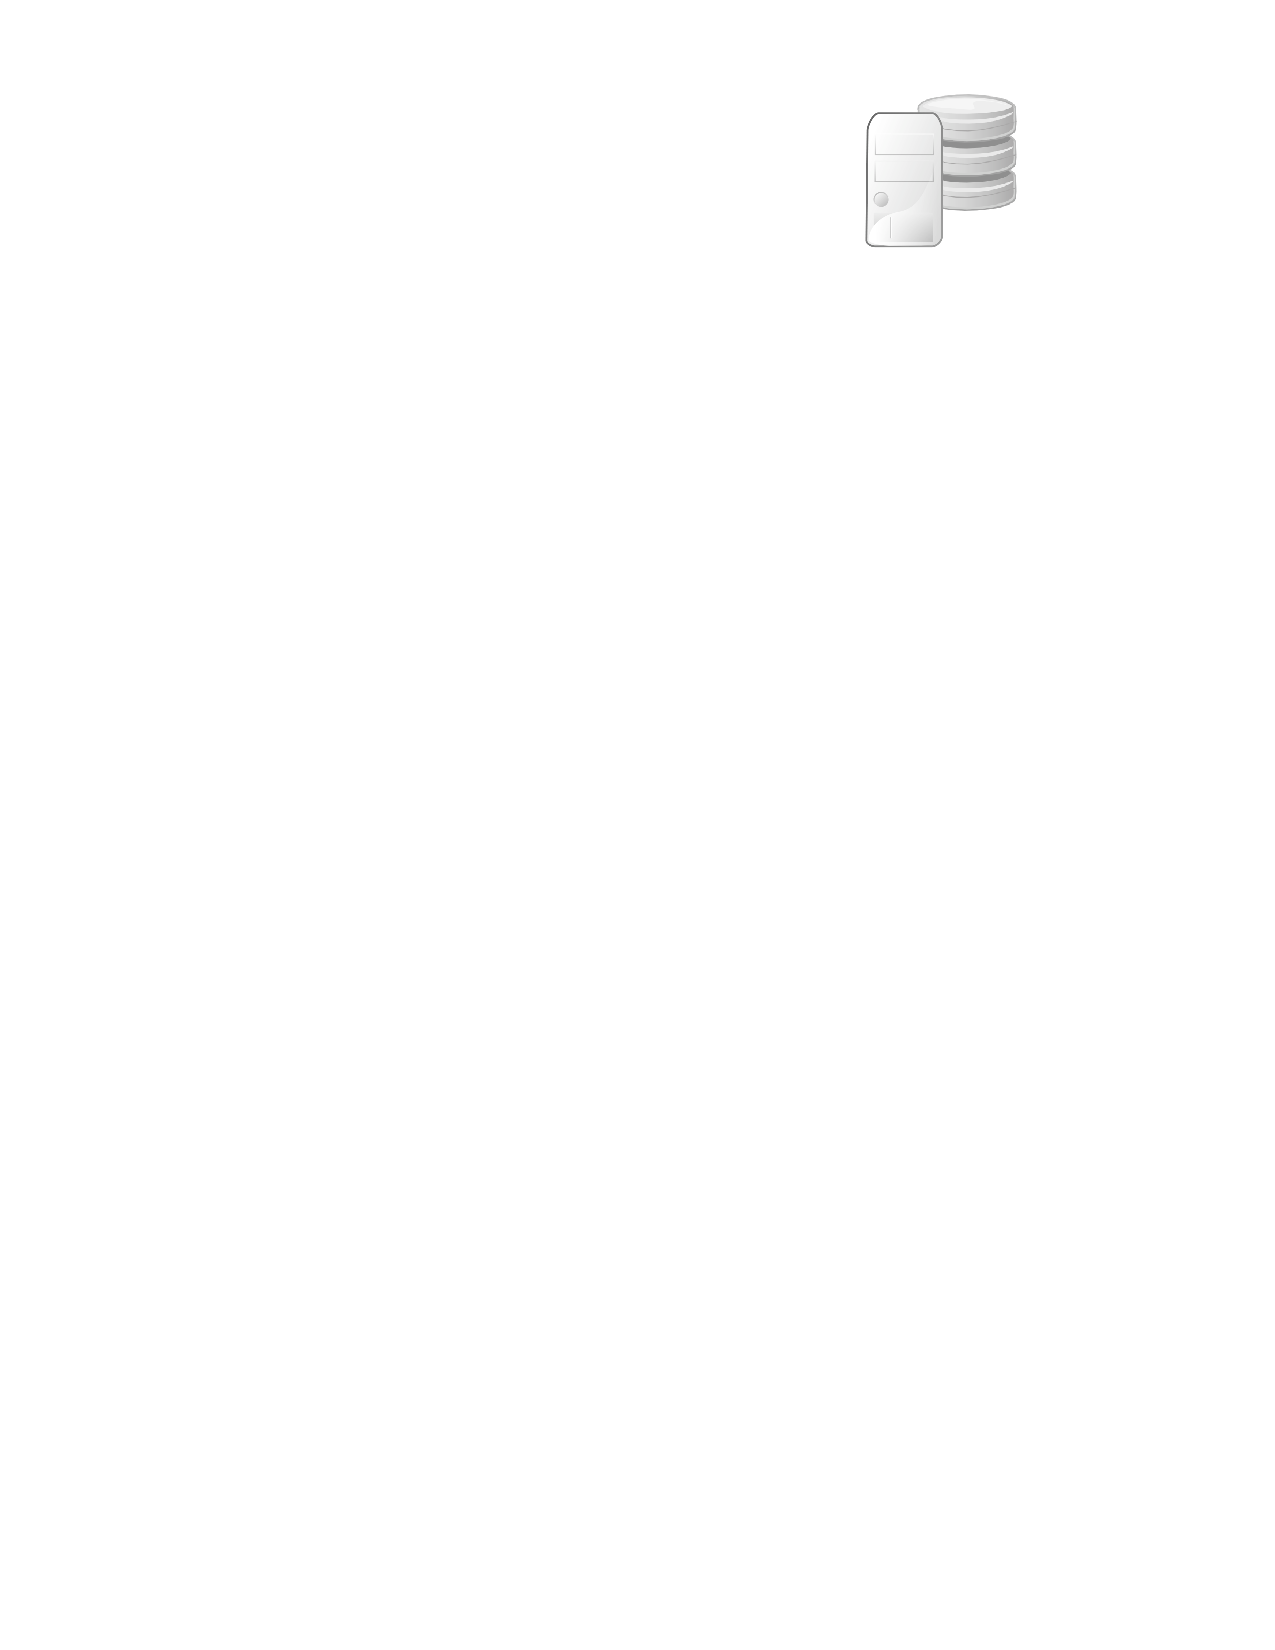
\includegraphics[height=\rinner]{figures/reposerver}\\\emph{Stratum 0 R/W}}};
	\draw[public] (0,0) circle (\router);
	
	\node[mirror] (cern) at (0,\router) {\parbox{\rmirror}{\small\centering CERN\\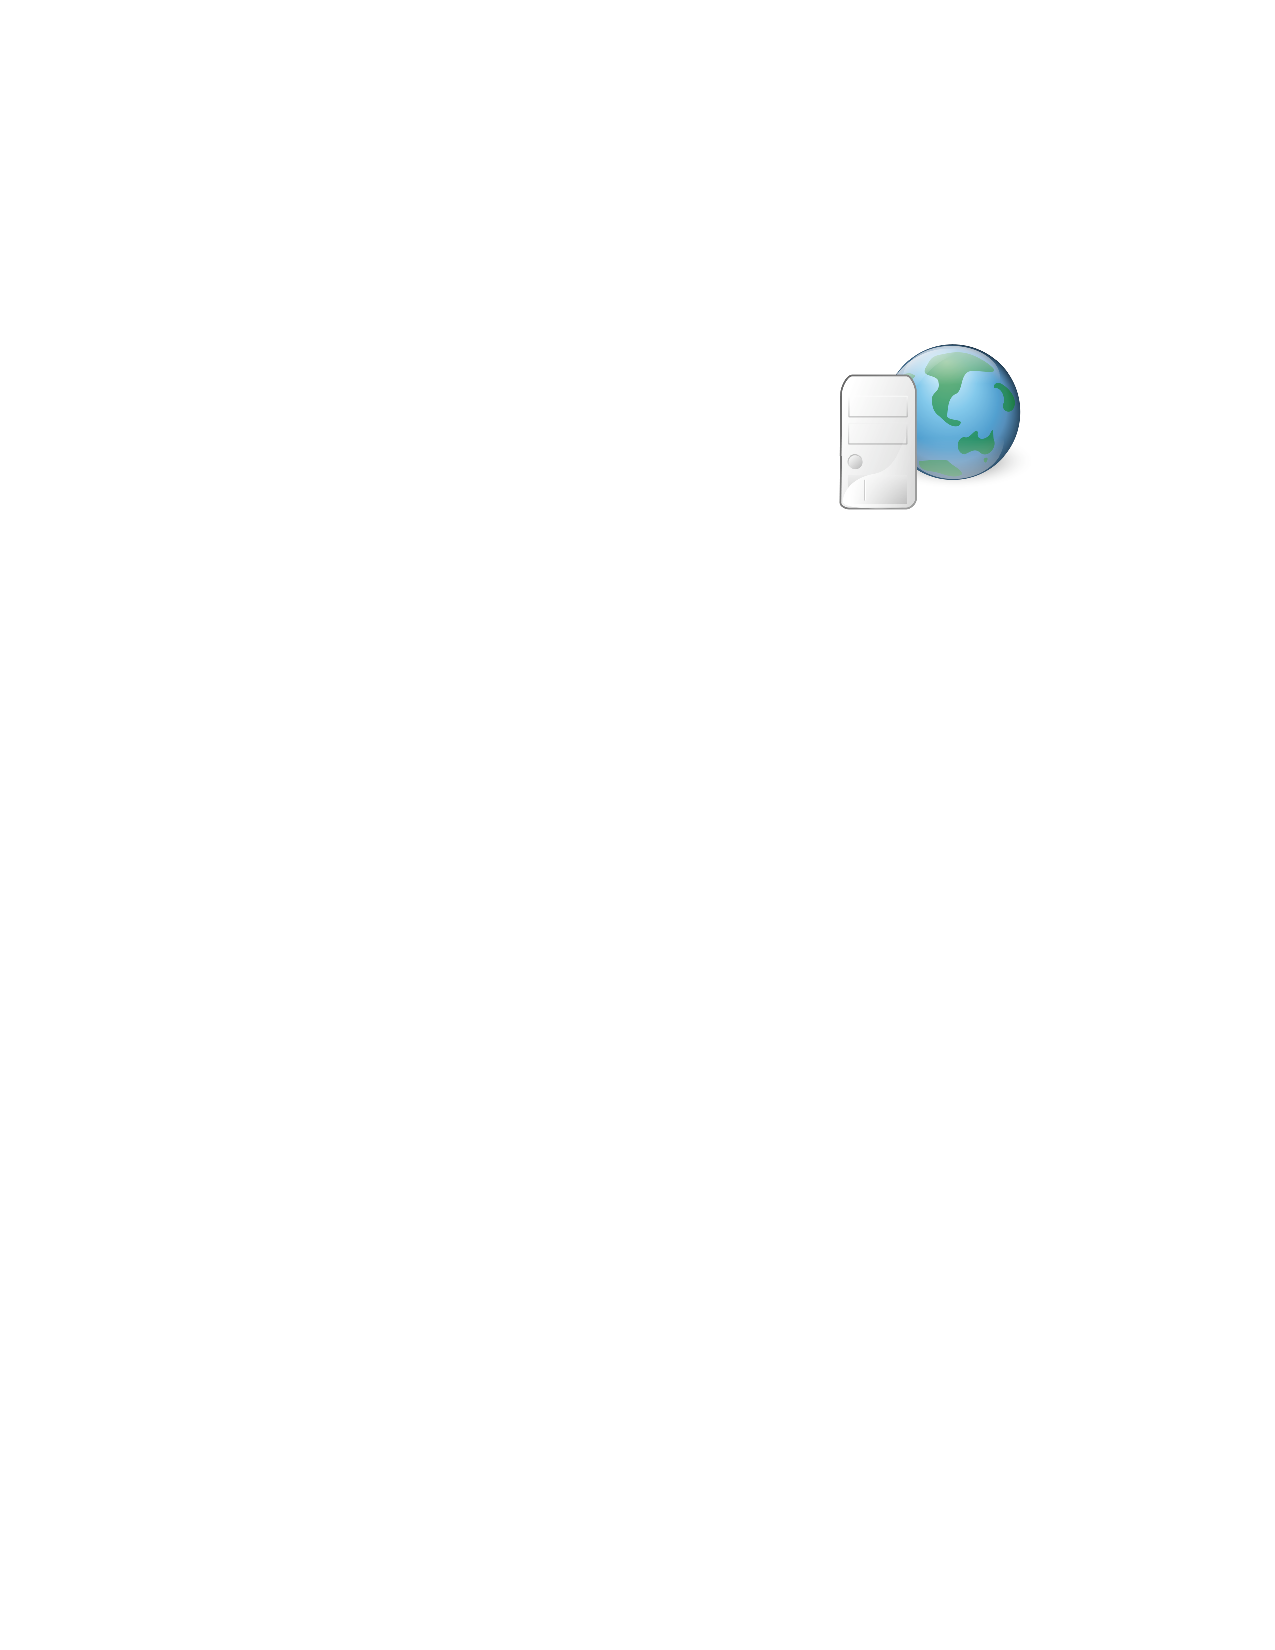
\includegraphics[height=\websize]{figures/webserver}}};
	%\draw[mirror] (cern) circle (\rmirror);
	\node[mirror] (ral) at (\router,0) {\parbox{\rmirror}{\small\centering RAL (U.K.)\\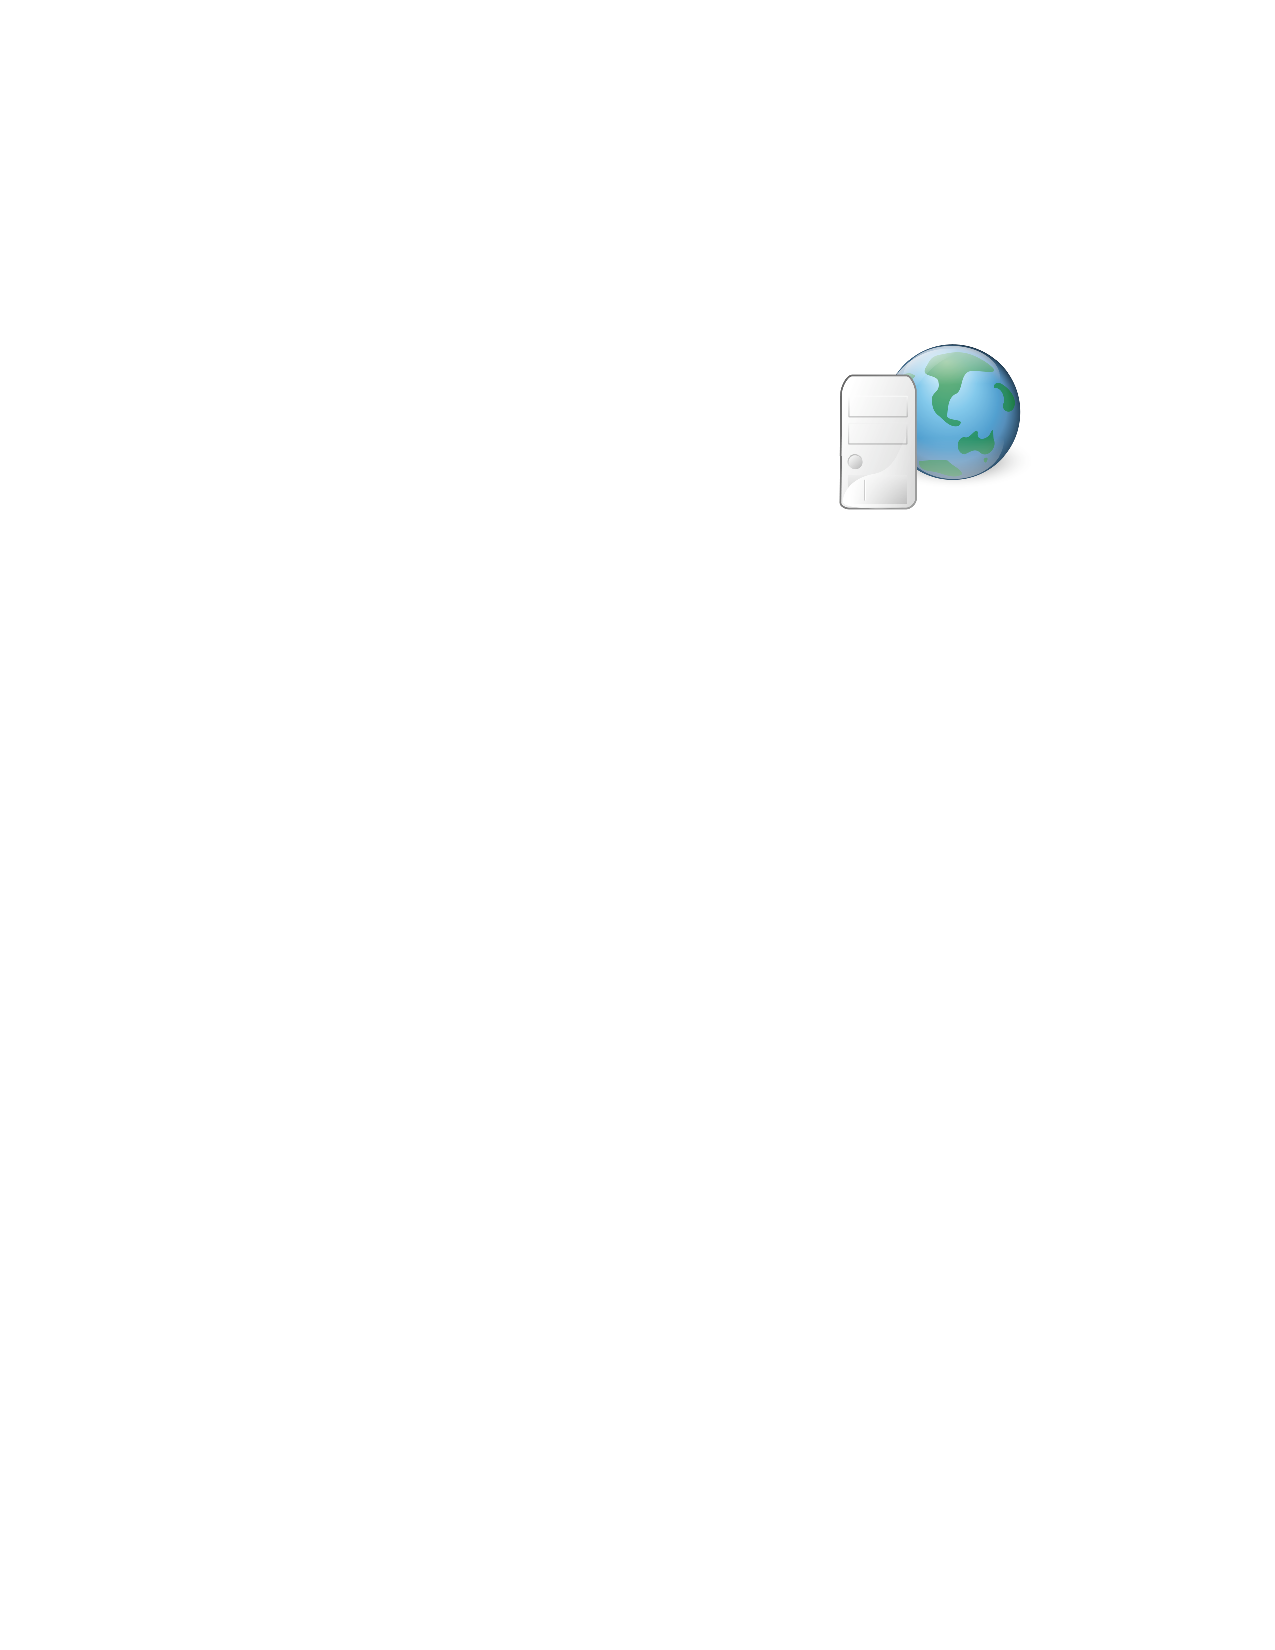
\includegraphics[height=\websize]{figures/webserver}}};
	%\draw[mirror] (ral) circle (\rmirror);
	\node[mirror] (bnl) at (-\router,0) {\parbox{\rmirror}{\small\centering FermiLab\\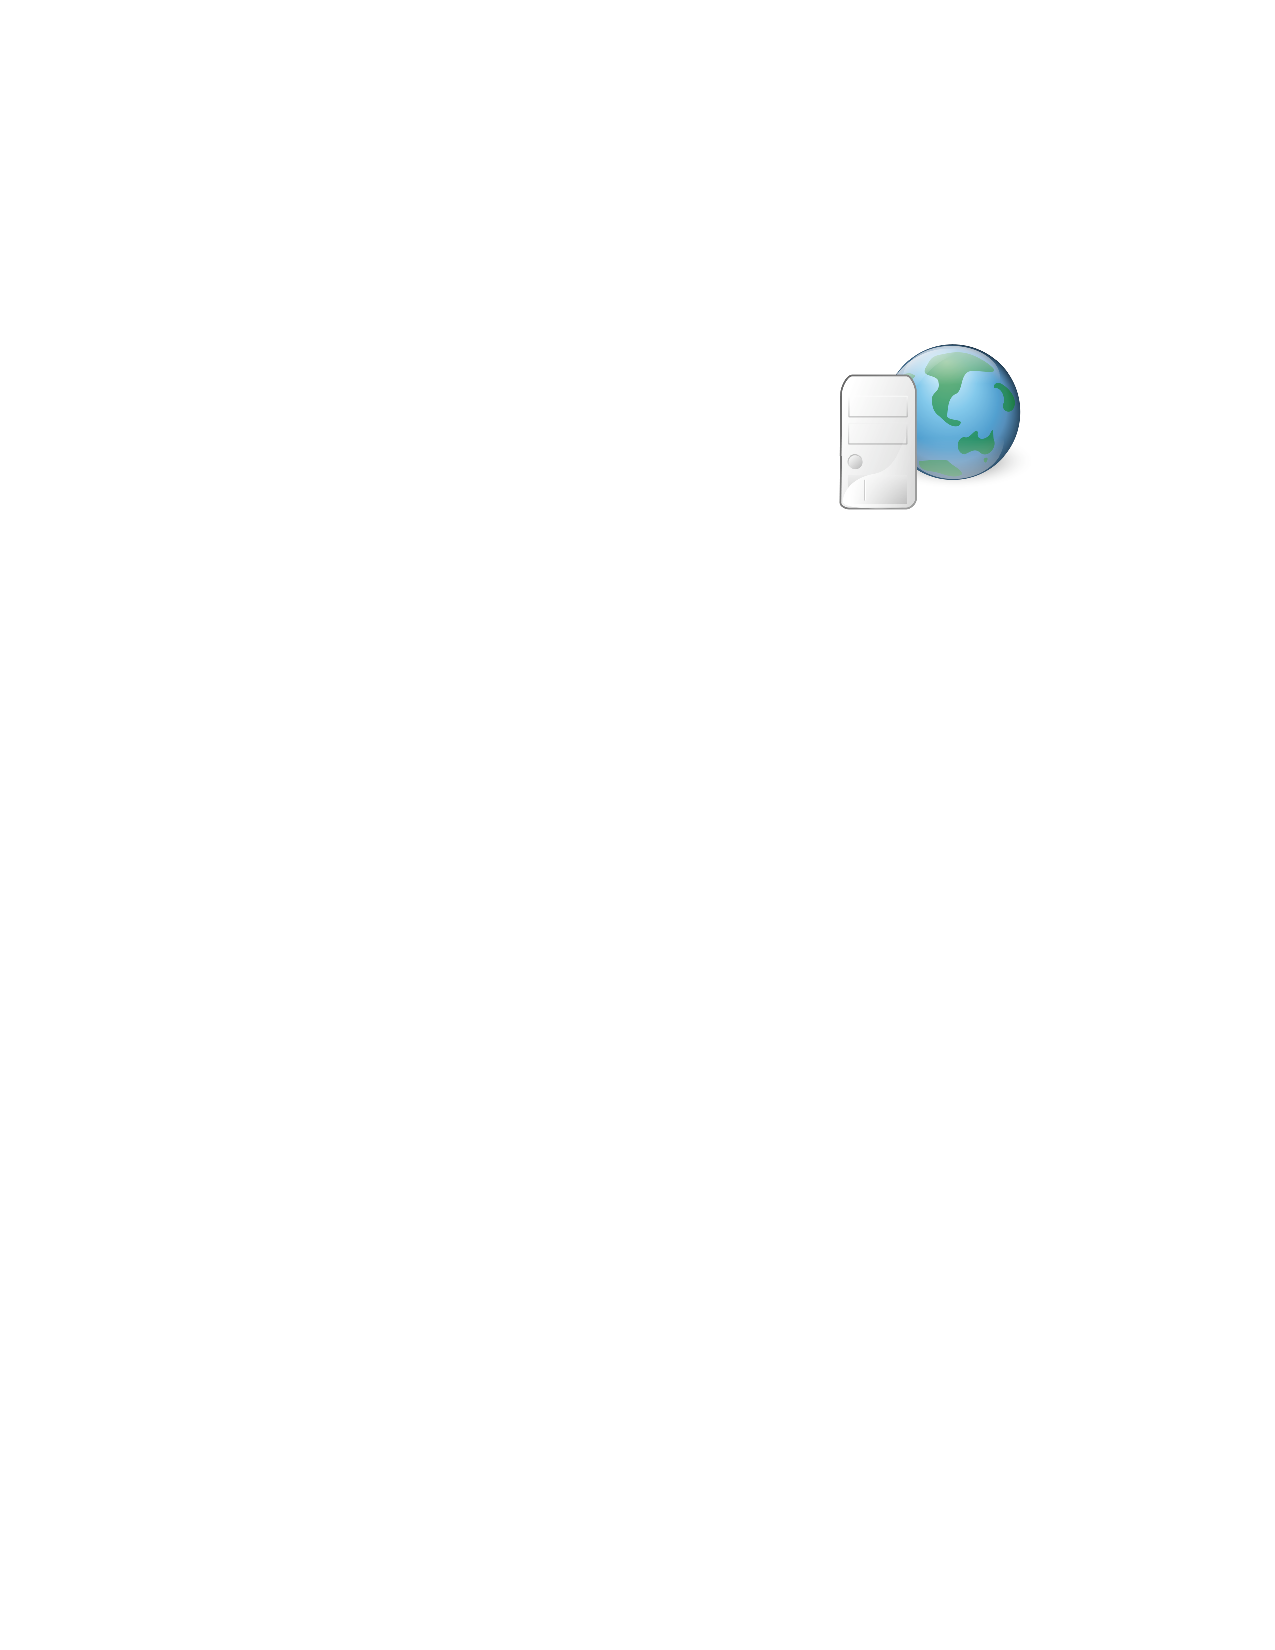
\includegraphics[height=\websize]{figures/webserver}}};
	\node[mirror] (fermilab) at (canvas polar cs:angle=225,radius=\router) {\parbox{\rmirror}{\small\centering BNL\\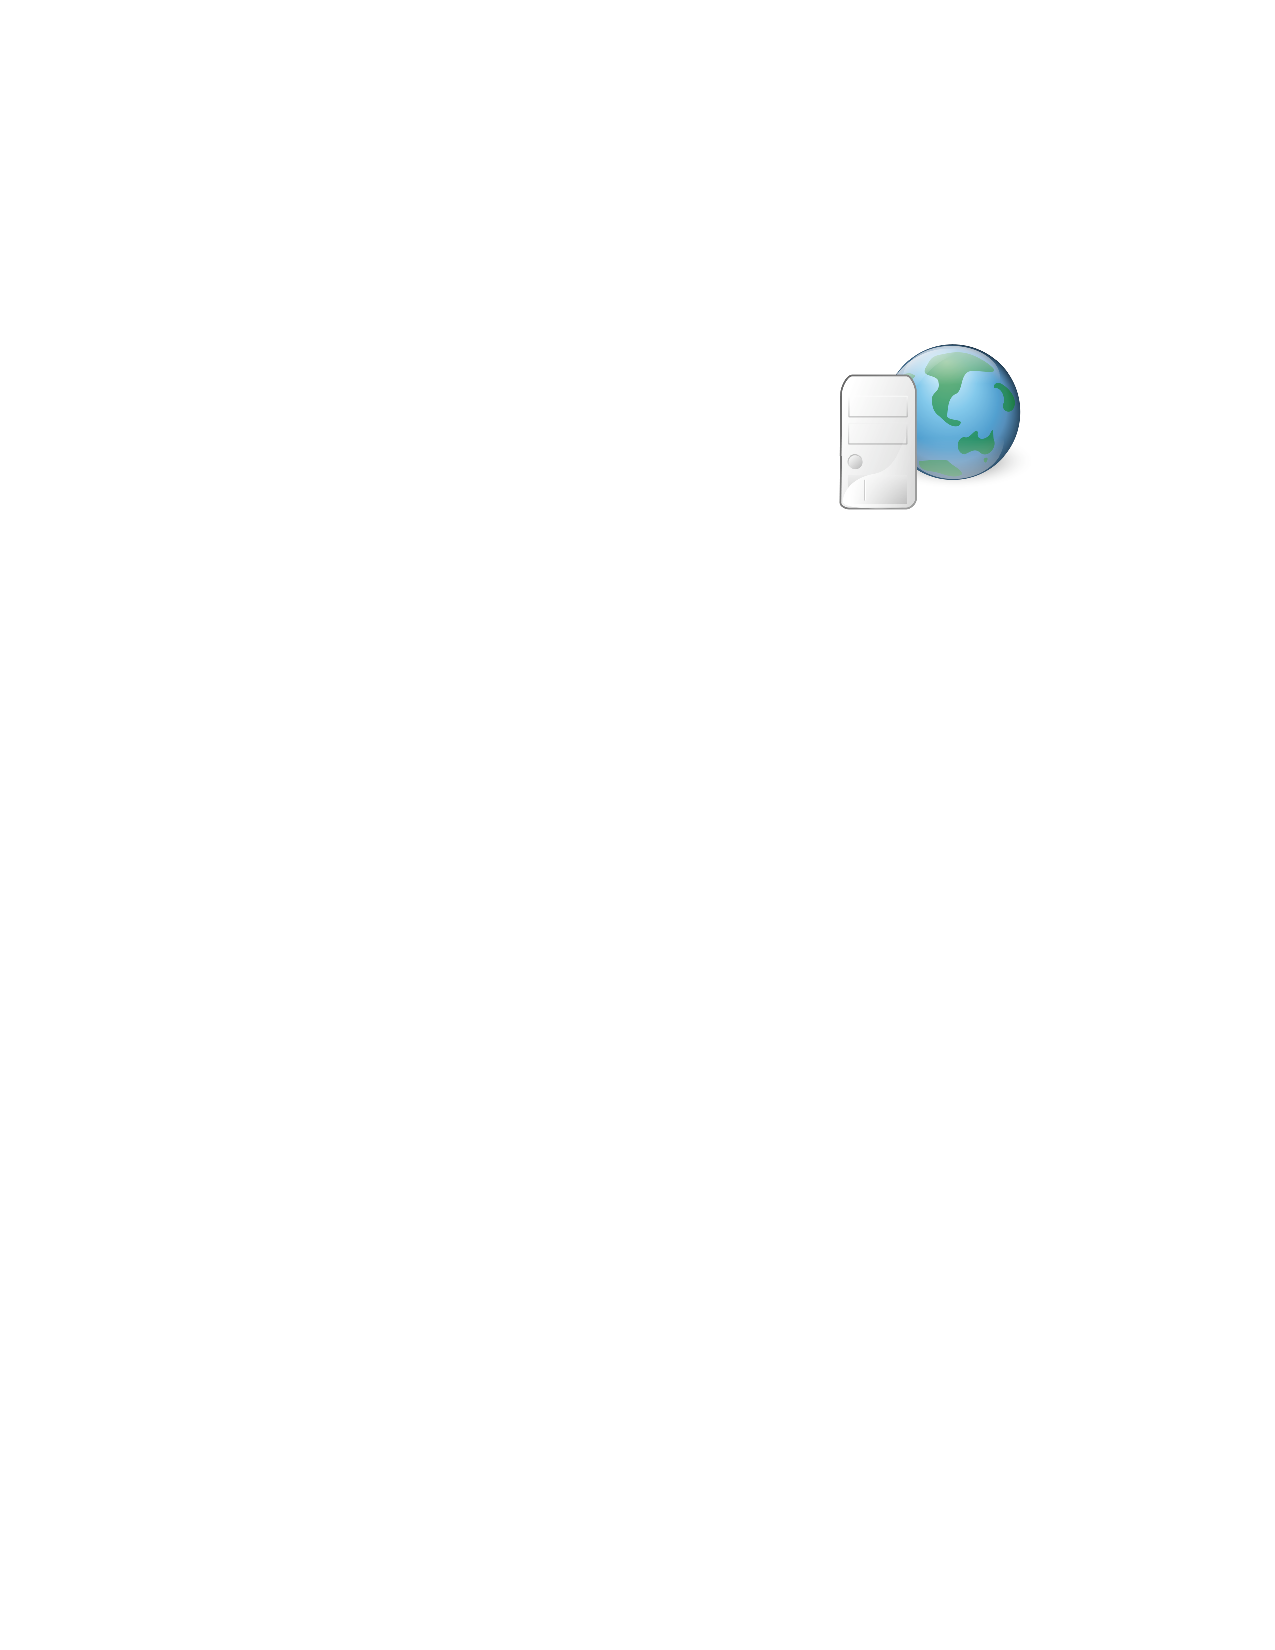
\includegraphics[height=\websize]{figures/webserver}}};
	\node[mirror] (desy) at (canvas polar cs:angle=-45,radius=\router) {\parbox{\rmirror}{\small\centering DESY\\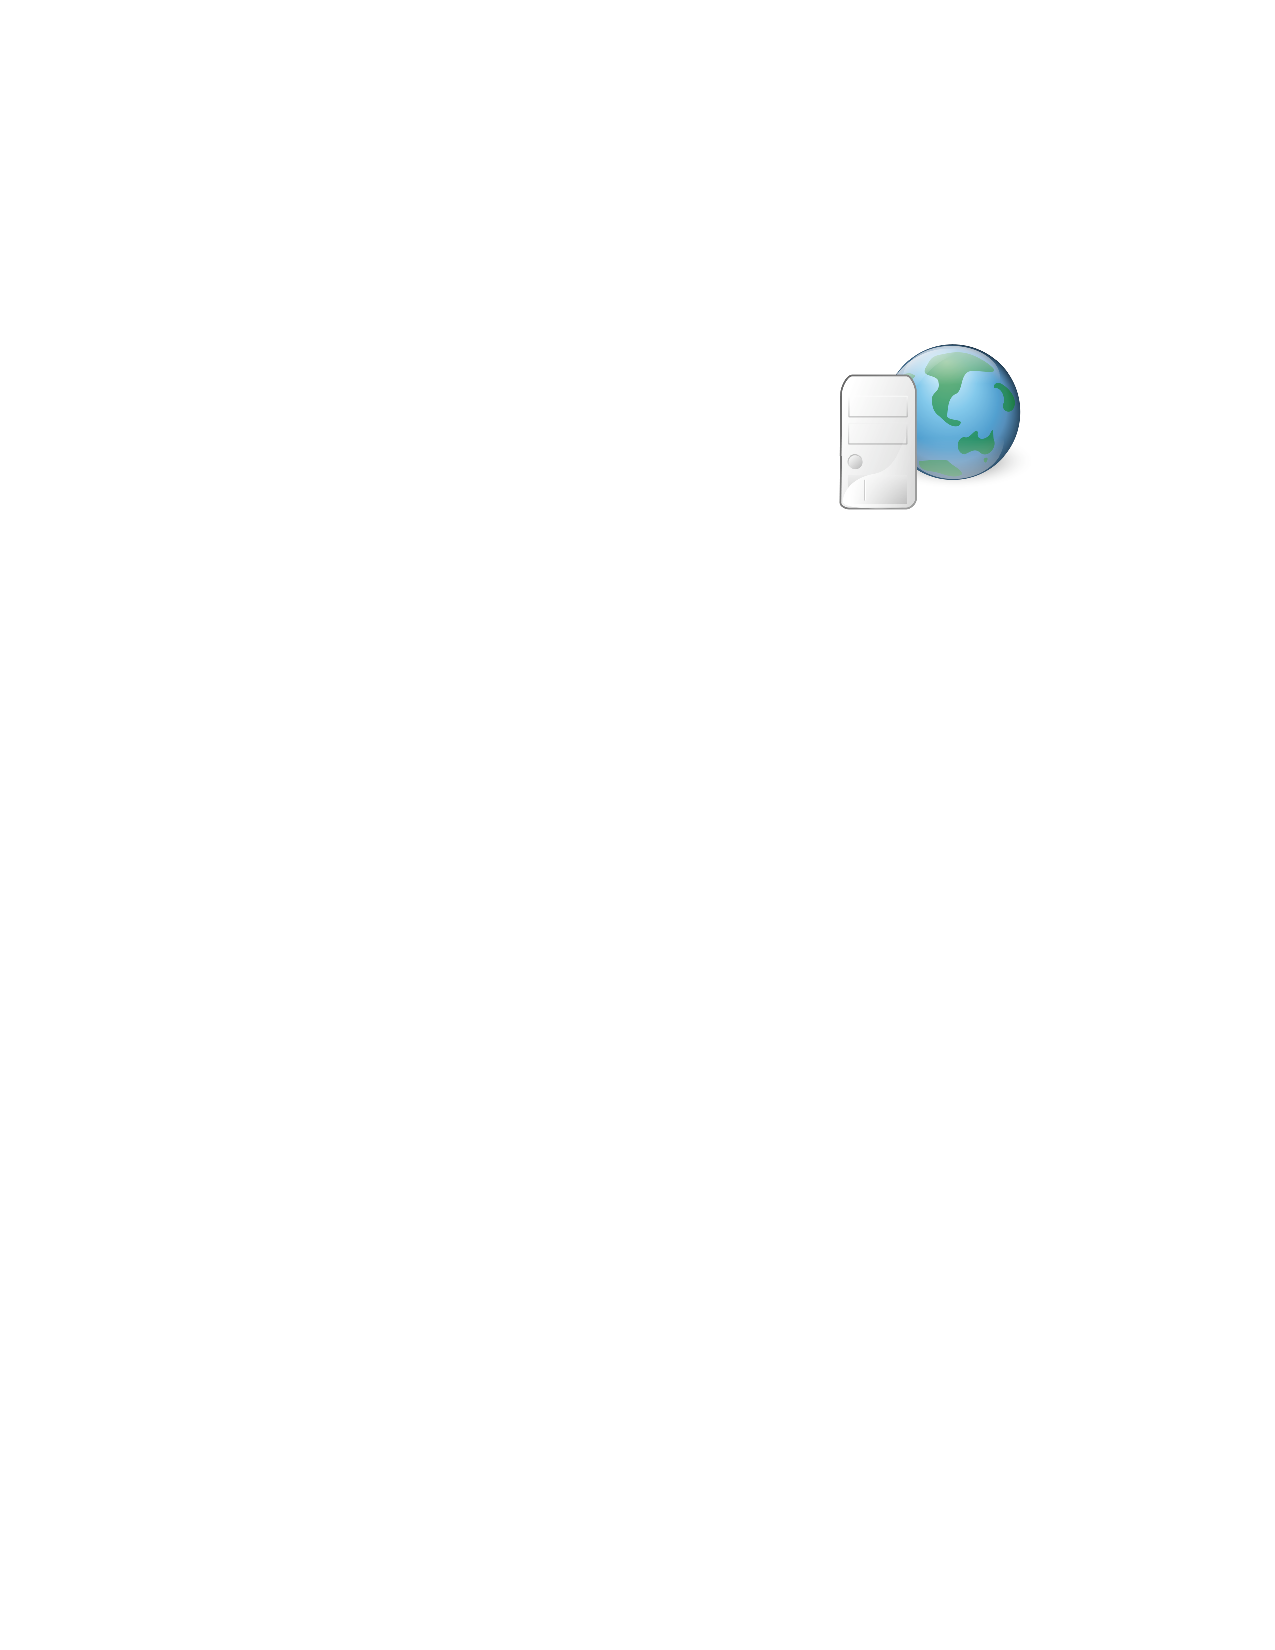
\includegraphics[height=\websize]{figures/webserver}}};
	\node[mirror] (nikhef) at (canvas polar cs:angle=45,radius=\router) {\parbox{\rmirror}{\small\centering NIKHEF\\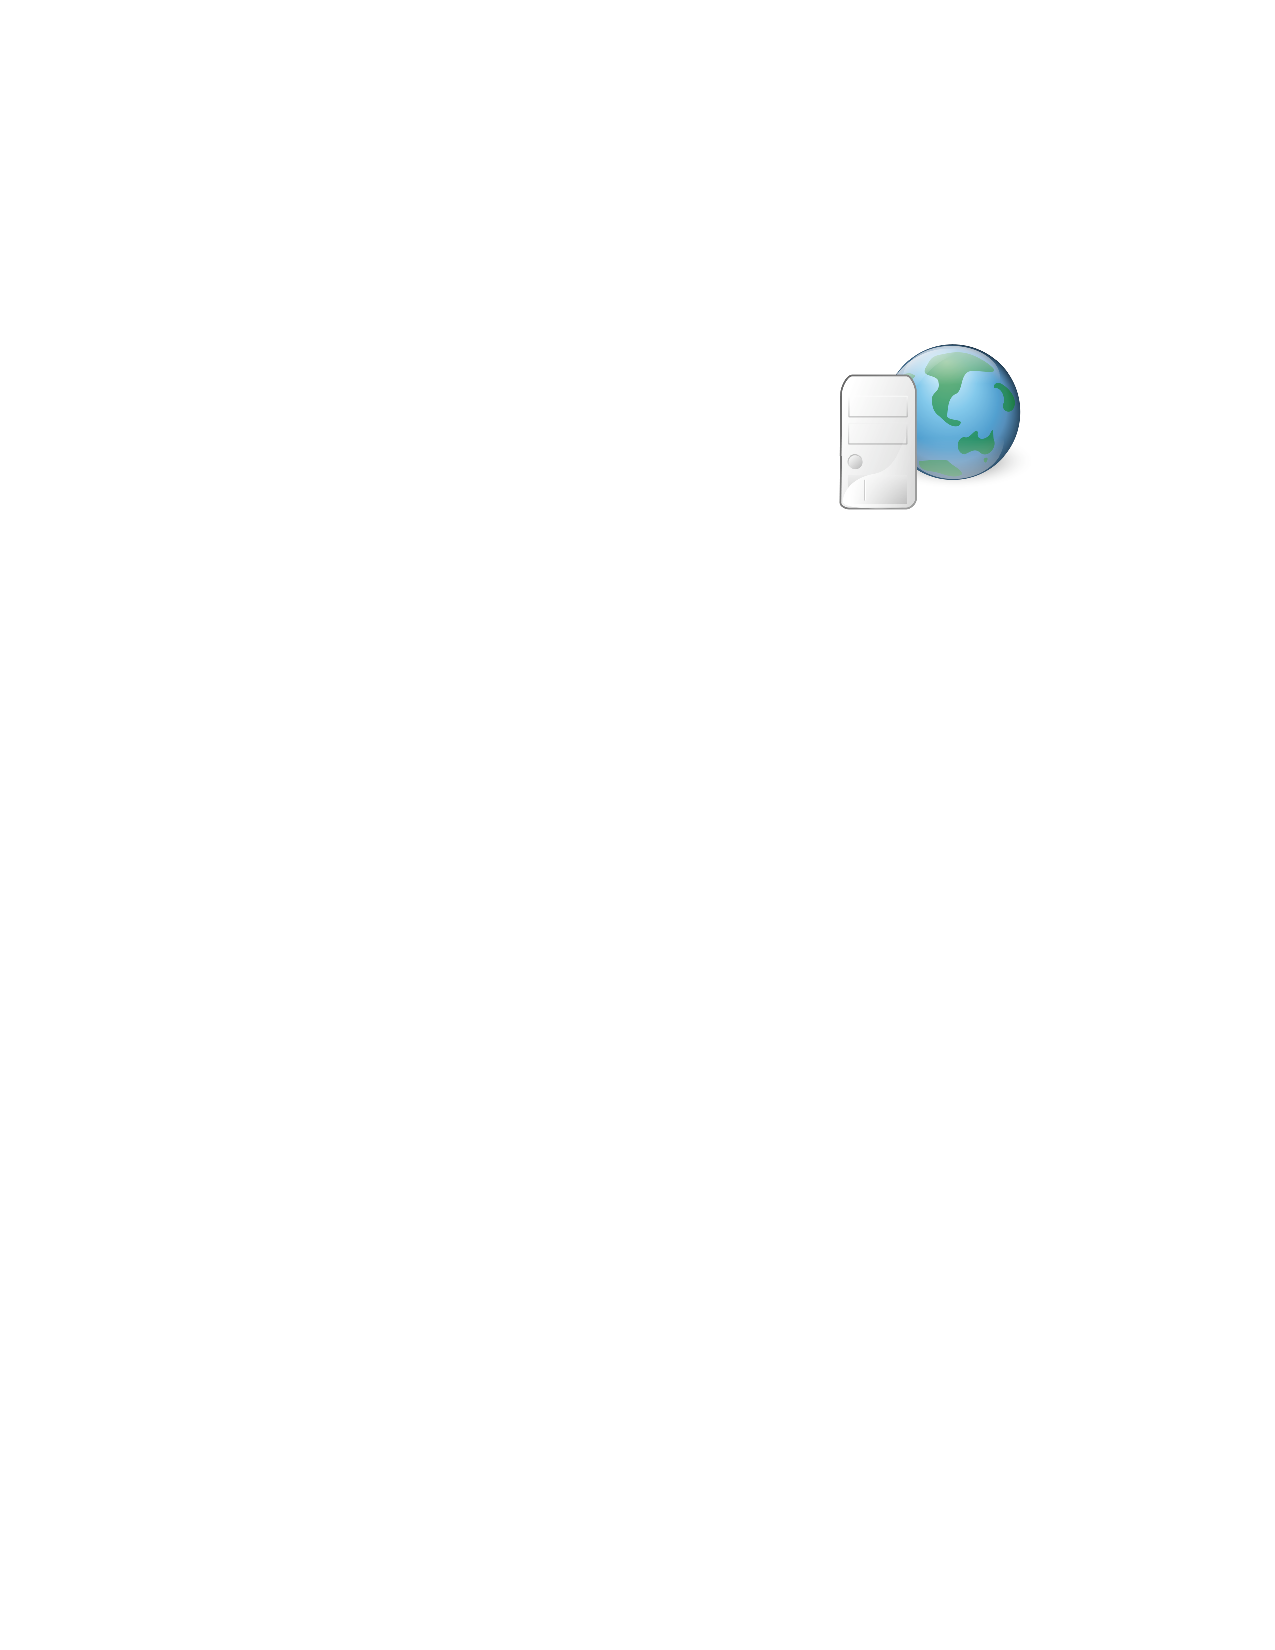
\includegraphics[height=\websize]{figures/webserver}}};
	%\draw[mirror] (bnl) circle (\rmirror);
	\node[mirror] (other) at (0,-\router) {\parbox{\rmirror}{\small\centering \emph{ASGC (Taiwan)}\\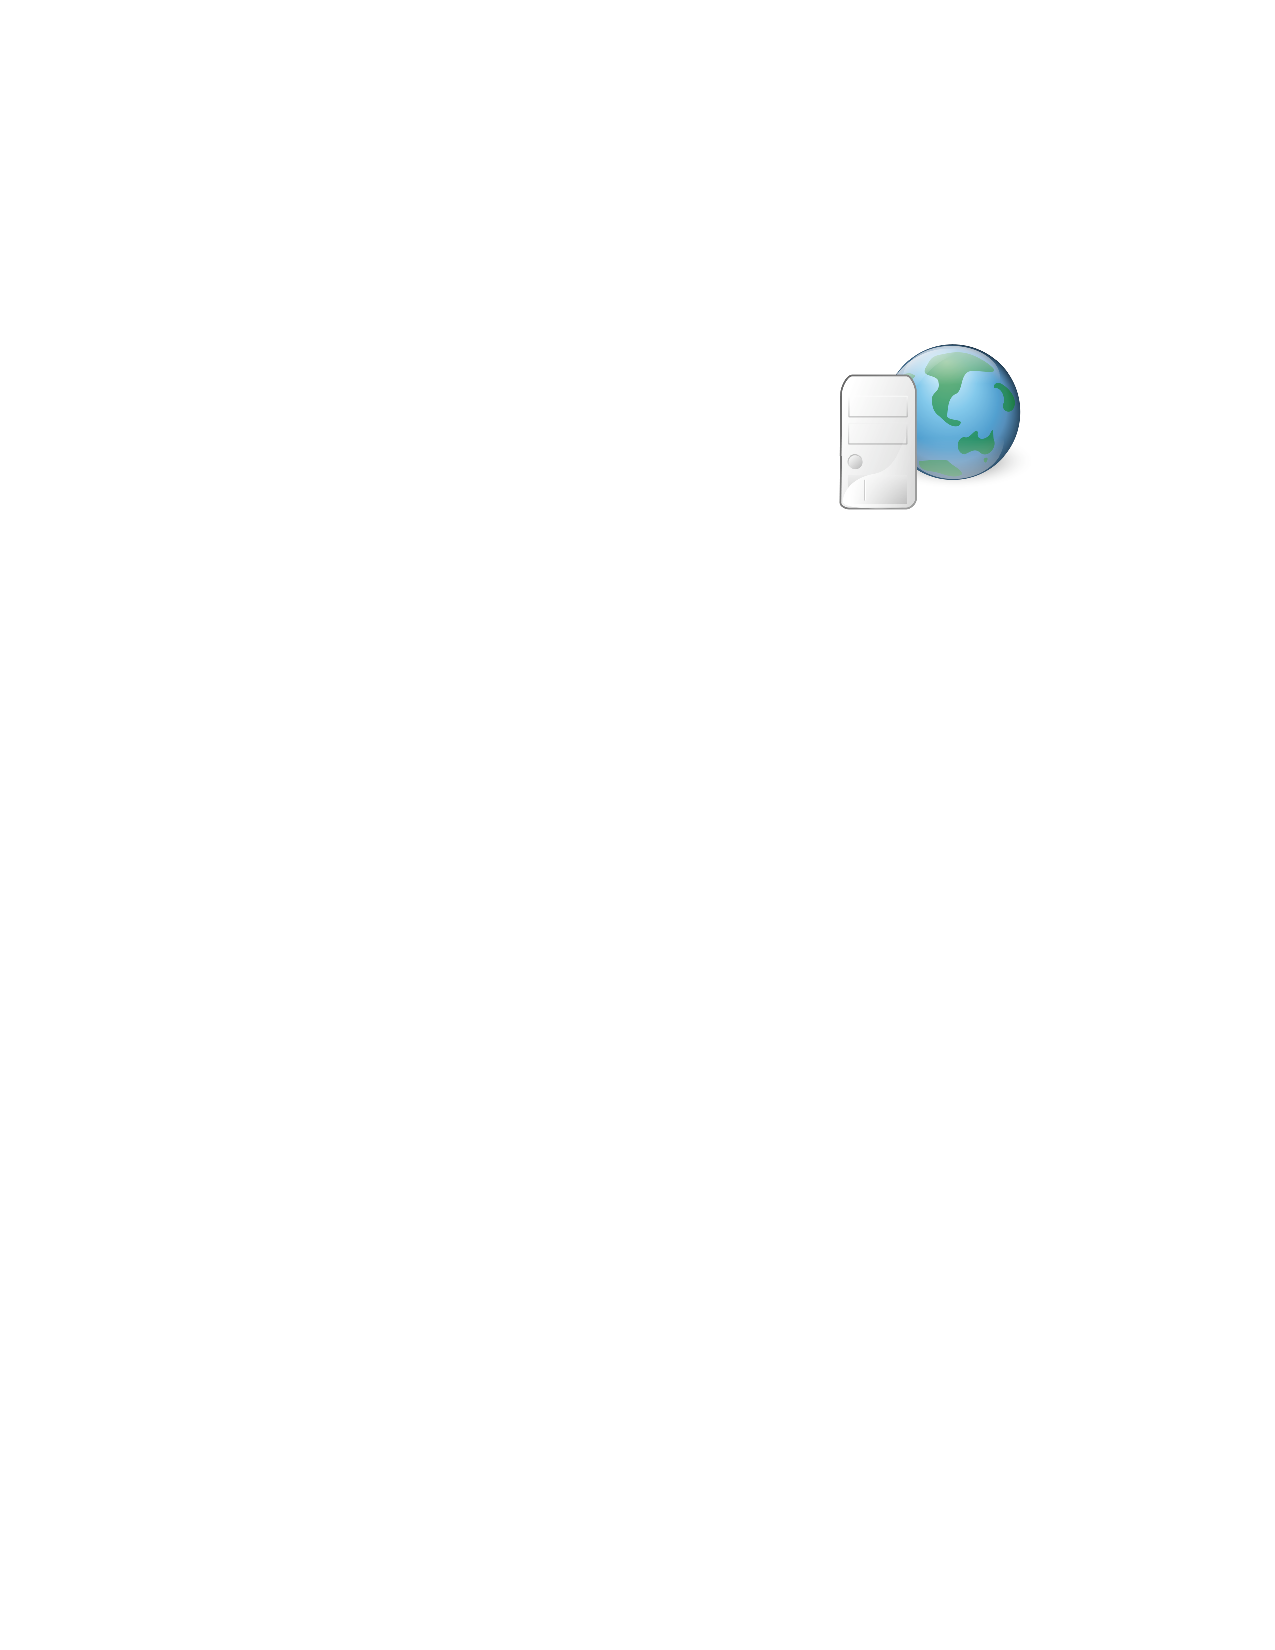
\includegraphics[height=\websize]{figures/webserver}}};
	%\draw[mirror] (other) circle (\rmirror);
	
	
	\draw[decorate,decoration={text along path,text color=blue,text={~~~~~~~~~~~~~~~~~~~|\small\it|Stratum 1||~}}] (-\router-0.3cm,0) arc (180:90:\router+0.3cm);
	\draw[decorate,decoration={text along path,text color=blue,text={~~~~~~~~~~~~~|\small|Public Mirrors||~}}] (-\router+0.5cm,0) arc (180:90:\router-0.5cm);
	%\draw (0,0) .. controls +(up:2cm) and +(left:2cm) .. (1,3) {node[public,sloped,above]{\emph{Stratum 1} Public Mirrors}};
	
	%\node[red,thick,fill=white,draw,cloud,aspect=1.5,xshift=\router+\rmirror+2cm] (tier1) {\parbox{2.2cm}{\centering\footnotesize\emph{Stratum 2}\\Private Replicas\\(Tier 1)}};
	
	\draw[replication] (rw) -- (cern);
	\draw[replication] (rw) -- (ral);
	\draw[replication] (rw) -- (bnl);
	\draw[replication] (rw) -- (fermilab);
	\draw[replication] (rw) -- (desy);
	\draw[replication] (rw) -- (nikhef);
	\draw[replication] (rw) -- (other);
	%\draw[replication,red] (ral) -- ($(tier1)-(1.8cm,0)$);
	
	\node[proxycolor,fill=white] at (-1.6*\router,0) {\parbox{1.5cm}{\centering\small Proxy\\Hierarchy}};
	\node[proxycolor,fill=white] at (1.6*\router,0) {\parbox{1.5cm}{\centering\small Proxy\\Hierarchy}};
	
\end{tikzpicture}

%\end{document}
}
	\end{center}
	\caption{\cvmfs\ content distribution network for the cern.ch domain: Stratum 1 replica servers are located in Europe, the U.S.\ and Asia.  
		One protected r/w instance (Stratum 0) is feeding up the public, distributed mirror servers. 
		A distributed hierarchy of proxy servers fetches content from the closest public mirror server.}
	\label{fig:stratum1}
\end{figure}

A Stratum~1 server is a standard web server that uses the \cvmfs\ server toolkit to create and maintain a mirror of a \cvmfs\ repository served by a Stratum~0 server.
To this end, the \texttt{cvmfs\_server} utility provides the \texttt{add-replica} command.
This command will register the Stratum~0 URL and prepare the local web server.
Periodical synchronization has to be scheduled, for instance with \texttt{cron}, using the \texttt{cvmfs\_server snapshot} command.
The advantage over general purpose mirroring tools such as \product{rSync} is that all \cvmfs\ file integrity verifications mechansims from the \fuse\ client are reused.
Additionally, by the aid of the \cvmfs\ file catalogs, the \texttt{cvmfs\_server} utility knows beforehand (without remote listing) which files to transfer.

In order to prevent accidental synchronization from a repository, the Stratum~0 repository maintainer has to create a \texttt{.cvmfs\_master\_replica} file in the HTTP root directory.
Also keep in mind that replication will thrash any caches that might be between Stratum~1 and Stratum~0.
A direct connection is therefore preferable.

\section{Recommended Setup}
The vast majority of HTTP requests will be served by the site's local proxy servers.
Being a publicly available service, however, we recommend to install caching \squid\ frontends in front of the Stratum~1 web server.
This setup is shown in Figure~\ref{fig:stratum1front}

\begin{figure}
	\centering
	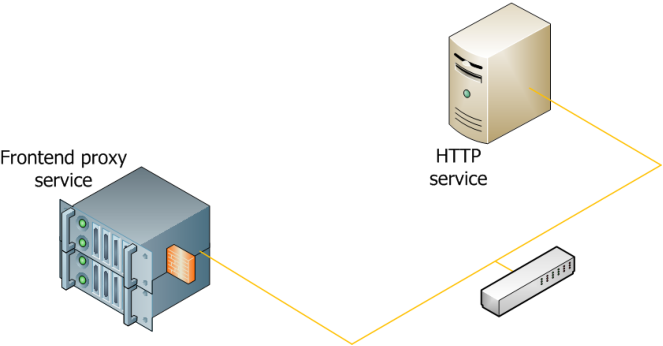
\includegraphics{figures/stratum1front}
	\caption{Recommended setup: 2 DNS load-balanced (round-robin) \squid\ machines in a reverse proxy mode in front of a single storage and web server.}
	\label{fig:stratum1front}
\end{figure}

We suggest the following key parameters:
\begin{description}
	\item[Storage.] 
		RAID-protected storage.
		The \texttt{cvmfs\_server} utility should have low latency to the storage because it runs a large number of system calls (\texttt{stat()}) against it.
		For the local storage backends ext3/4 filesystems are preferred (rather than XFS).
	\item[Web server.]
		A standard Apache server.
		Directory listing is not required.
		In addition, it is a good practice to exclude search engines from the replica web server by an appropriate robots.txt.
		The work load is mainly covered by the \squid\ servers, hence performance of the web server is not critical.
		However, the webserver should be close to the storage in terms of latency.
	\item[Squid frontend.]
		At least 2 \squid\ servers configured in load-balance mode as reverse proxies for the web server.
		The Squid frontends should listen on ports 80 and 8000.
		The more RAM \squid\ can use for caching, the better.
\end{description}

\section{Squid Configuration}
The \squid\ configuration differs from the site-local Squids because the Stratum~1 \squid\ servers are transparent to the clients (\emph{reverse proxy}).
The Squid server is configured as reverse proxy for the web server.
Concurrent requests for the same URL should be collapsed into one request to the backend.
Additionally, the cache sizes have to be set.
As the expiry rules are set by the web server, \squid\ cache expiry rules remain unchanged.

The following lines should appear accordingly in /etc/squid/squid.conf:
\begin{verbatim}
  http_port 80 accel
  http_port 8000 accel
  http_access allow all
  cache_peer <APACHE_HOSTNAME> parent 80 0 no-query originserver
  collapsed_forwarding on

  max_filedesc 8192

  cache_mem <MEM_CACHE_SIZE> MB
  cache_dir aufs /var/spool/squid <DISK_CACHE_SIZE in MB> 32 256
  maximum_object_size 1024 MB
  maximum_object_size_in_memory 8 MB
\end{verbatim}
\quad\\
Note that \texttt{http\_access allow all} has to be inserted before (or instead of) the line \texttt{http\_access deny all}.

Check the configuration syntax by \texttt{squid -k parse}.
Create the hard disk cache area with \texttt{squid -z}. 
In order to make the increased number of file descriptors effective for \squid, execute \texttt{ulimit -n 8192} prior to starting the squid service.

\section{Monitoring}
The \texttt{cvmfs\_server} utility reports status and problems to \texttt{stdout} and \texttt{stderr}.

For the infrastructure, standard \nagios\ HTTP checks do the job.
Configure it with the URL \url{http://$replica-server/cvmfs/$repository_name/.cvmfspublished}.
This file can also be used to monitor if the same repository revision is served by the Stratum~0 server and all the Stratum~1 servers.
In order to tune the hardware and cache sizes, keep an eye on the Squid server's CPU and I/O load.

Keep an eye on HTTP 404 errors.
For normal CernVM-FS traffic, such failures should not occur.
Traffic from \cvmfs\ clients is marked by an \texttt{X-CVMFS2} header.
